\subsection{Example \#5: single time series analysis with interventions}
\label{S:Example_DISP_intervention}
\subsubsection{Data description}
This case is based on Example \#1 (see \ref{S:Example_DISP}) where we removed some part of the data and introduce discrete shifts into it. This example illustrates what typically happens a sensor fails; when a sensor fails, the data start to be missing (i.e. \lstinline[basicstyle = \mlttfamily \small, backgroundcolor = \color{light-gray}]!NaN!) and it often takes from several weeks to several months before the sensor is replaced. When the sensor is replaced, it is in most cases re-initialized at a different initial value than the previous sensor which lead to a discrete shift in the time series, as depicted in Figure~\ref{fig:DataSummary1}. Here in addition to the components employed for Example \#1, we also employ a Local intervention in order to estimate the magnitude of the corrections require to eliminate the discrete shifts created by sensor replacement.

Note that again, in this example, we choose to resample the original data in order to have a timesteps of 6h instead of 1h. 

\begin{figure*}[h]
\centering
\begin{subfigure}{\linewidth}
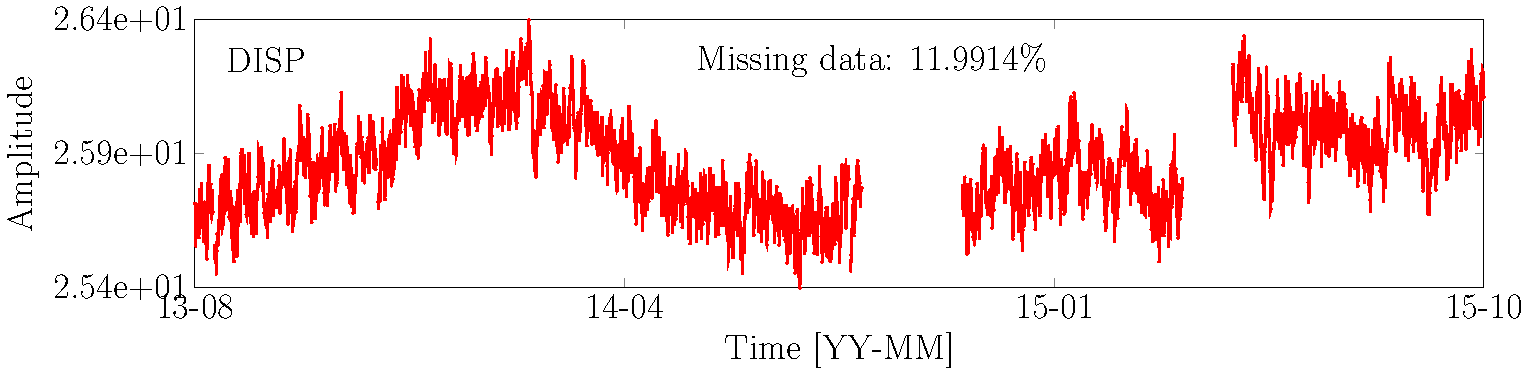
\includegraphics[width=0.95\linewidth]{./docfigs/Example_DISP_INTERVENTION/ALL_AMPLITUDES.pdf}
\caption{Amplitude}
\end{subfigure}
\begin{subfigure}{\linewidth}
\centering
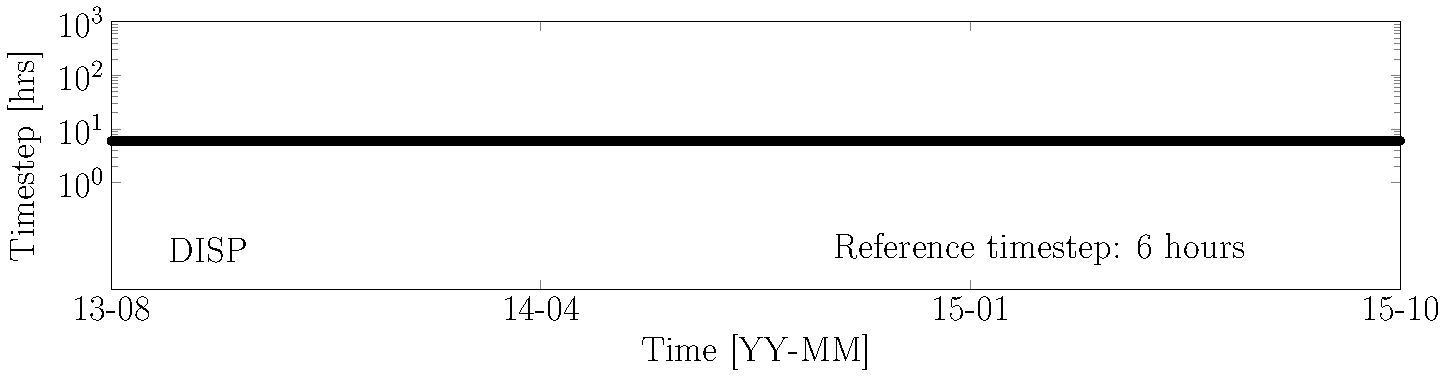
\includegraphics[width=0.9\linewidth]{./docfigs/Example_DISP_INTERVENTION/ALL_TIMESTEPS.pdf} 
\caption{Timestep}
\end{subfigure}
\begin{subfigure}{\linewidth}
\centering
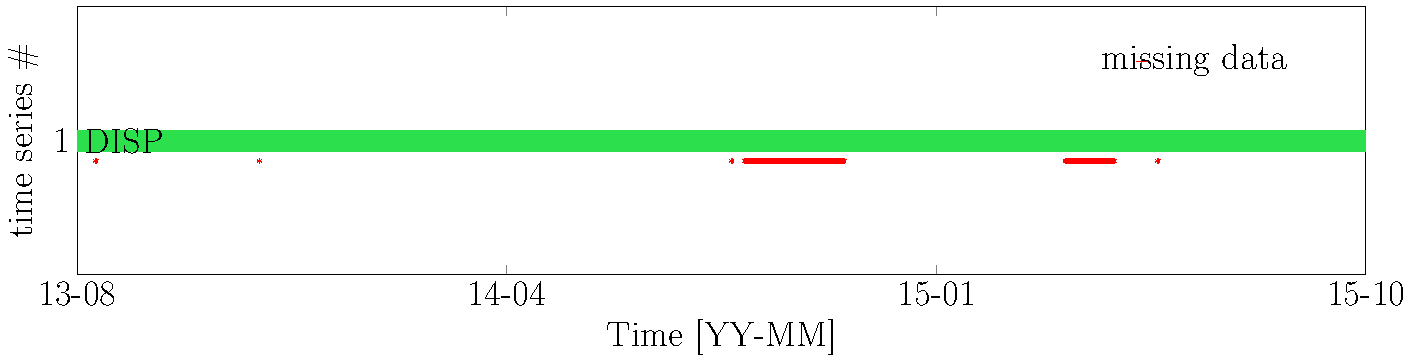
\includegraphics[width=0.9\linewidth]{./docfigs/Example_DISP_INTERVENTION/AVAILABILITY.pdf}
\caption{Availability}
\end{subfigure}
\caption{Raw data in the example \#1 where the reference timestep is 1h.}
\label{fig:DataSummary1}
\end{figure*}


\subsubsection{Model description}
\label{SS:ModelConstructionExample1}
The model includes one model class, and the hidden states variables are 
\begin{gather*}
\textbf{x}=[x^{\mathtt{LL}}, x^{\mathtt{P1}\text{,yearly}}, x^{\mathtt{P2}\text{,yearly}}, x^{\mathtt{P1}\text{,daily}}, x^{\mathtt{P2}\text{,daily}}, x^{\mathtt{AR}}, x^{\mathtt{LI}}].
\end{gather*}
When using a Level intervention component, the user must provide discrete timestamps where it is required to estimate the magnitude of a discrete shift in the dataset (see \S\ref{SSS:LI}). A user can do so by specifying in the configuration file \colorbox{light-gray}{\lstinline[basicstyle = \mlttfamily \small, backgroundcolor = \color{light-gray}]!data.interventions=[t_{1}, t_{2}, ... , t_{n}]!}. The configuration file for this problem is presented in the Listing \ref{LST:CFGFileExampleInt} where the timestamps where the shift occur are \colorbox{light-gray}{\lstinline[basicstyle = \mlttfamily \small, backgroundcolor = \color{light-gray}]!data.interventions=[735929.875, 736099.875];!}. 

\begin{lstlisting}[linewidth=\linewidth, style=Matlab-editor,  basicstyle = \mlttfamily \tiny, backgroundcolor = \color{matlab-yellow}, caption = {Configuration file for the example \#5}, label=LST:CFGFileExampleInt, captionpos=b, float=h!]
%%%%%%%%%%%%%%%%%%%%%%%%%%%%%%%%%%%%%%%%%%%%%%%%%%%%%%%%%%%%%%%%%%%%%%%%%%%
%% A - Project name
%%%%%%%%%%%%%%%%%%%%%%%%%%%%%%%%%%%%%%%%%%%%%%%%%%%%%%%%%%%%%%%%%%%%%%%%%%%
misc.ProjectName='Example_DISP_INTERVENTION';
%%%%%%%%%%%%%%%%%%%%%%%%%%%%%%%%%%%%%%%%%%%%%%%%%%%%%%%%%%%%%%%%%%%%%%%%%%%
%% B - Data
%%%%%%%%%%%%%%%%%%%%%%%%%%%%%%%%%%%%%%%%%%%%%%%%%%%%%%%%%%%%%%%%%%%%%%%%%%%
dat=load('DATA_Example_DISP_INTERVENTION.mat'); 
data.values=dat.values;
data.timestamps=dat.timestamps;
data.labels={'DISP'};
data.interventions=[735929.875, 736099.875];
%%%%%%%%%%%%%%%%%%%%%%%%%%%%%%%%%%%%%%%%%%%%%%%%%%%%%%%%%%%%%%%%%%%%%%%%%%%
%% C - Model structure 
%%%%%%%%%%%%%%%%%%%%%%%%%%%%%%%%%%%%%%%%%%%%%%%%%%%%%%%%%%%%%%%%%%%%%%%%%%%
% Components reference numbers
% 11: Local level
% 12: Local trend
% 13: Local acceleration
% 21: Local level compatible with local trend
% 22: Local level compatible with local acceleration
% 23: Local trend compatible with local acceleration
% 31: Periodic
% 41: Autoregressive
% 51: Kernel regression
% 61: Level Intervention

% Model components
model.components.block{1}={[11 31 31 41 61 ] };
 
% Model inter-components dependence | {[components form dataset_i depends on components from  dataset_j]_i,[...]}
model.components.ic={[ ] };
%%%%%%%%%%%%%%%%%%%%%%%%%%%%%%%%%%%%%%%%%%%%%%%%%%%%%%%%%%%%%%%%%%%%%%%%%%%
%% D - Model parameters 
%%%%%%%%%%%%%%%%%%%%%%%%%%%%%%%%%%%%%%%%%%%%%%%%%%%%%%%%%%%%%%%%%%%%%%%%%%%
model.param_properties={
     % #1           #2             #3      #4    #5               #6           #7       #8              #9              #10
     % Param name   Block name     Model   Obs   Bound            Prior        Mean     Std             Values          Ref
     '\sigma_w',   'LL',           '1',   '1',   [NaN  NaN  ],    'N/A',       NaN,     NaN,            0,              1      %#1   
     'p',          'PD1',          '1',   '1',   [NaN  NaN  ],    'N/A',       NaN,     NaN,            365.2422,       2      %#2   
     '\sigma_w',   'PD1',          '1',   '1',   [NaN  NaN  ],    'N/A',       NaN,     NaN,            0,              3      %#3   
     'p',          'PD2',          '1',   '1',   [NaN  NaN  ],    'N/A',       NaN,     NaN,            1,              4      %#4   
     '\sigma_w',   'PD2',          '1',   '1',   [NaN  NaN  ],    'N/A',       NaN,     NaN,            0,              5      %#5   
     '\phi',       'AR',           '1',   '1',   [0  1      ],    'N/A',       NaN,     NaN,            0.90399,        6      %#6   
     '\sigma_w',   'AR',           '1',   '1',   [0  Inf    ],    'N/A',       NaN,     NaN,            0.035428,       7      %#7   
     '\mu_b',      'LI',           '1',   '1',   [NaN  NaN  ],    'N/A',       NaN,     NaN,            0,              8      %#8   
     '\sigma_b',   'LI',           '1',   '1',   [NaN  NaN  ],    'N/A',       NaN,     NaN,            0.16276,        9      %#9   
     '\sigma_v',   '',             '1',   '1',   [0  Inf    ],    'N/A',       NaN,     NaN,            6.193e-06,      10     %#10  
};
%%%%%%%%%%%%%%%%%%%%%%%%%%%%%%%%%%%%%%%%%%%%%%%%%%%%%%%%%%%%%%%%%%%%%%%%%%%
%% E - Initial states values 
%%%%%%%%%%%%%%%%%%%%%%%%%%%%%%%%%%%%%%%%%%%%%%%%%%%%%%%%%%%%%%%%%%%%%%%%%%%
% Initial hidden states mean for model 1:
model.initX{ 1 }=[	25.9  	-0.194	-0.01 	-0.00411	0.0551	-0.0127	0     ]';
% Initial hidden states variance for model 1: 
model.initV{ 1 }=diag([ 	8.26E-05	0.000143	0.000106	4.86E-07	4.86E-07	0.00167	1E-20  ]);
% Initial probability for model 1
model.initS{1}=[1     ];

\end{lstlisting}

The model parameters associated with this model are
\begin{gather*}
\bm\theta=[\sigma_{w}^{\mathtt{LL}}, p^{\mathtt{P}, \text{yearly}}, \sigma_{w}^{\mathtt{P}, \text{yearly}} , p^{\mathtt{P}, \text{daily}}, \sigma_{w}^{\mathtt{P}, \text{daily}}, \phi^{\mathtt{AR}}, \sigma_{w}^{\mathtt{AR}}, \mu_{b}^{\mathtt{LI}}, \sigma_{b}^{\mathtt{LI}}, \sigma_{v}].
\end{gather*}
The optimized model parameters values computed using the Newton-Raphson algorithm (see~\ref{SS:THModelParameterEstimation}) with a training period of 180 days  are
\begin{gather*}
\bm\theta^{\text{*}}=[0, 365.2422, 0, 1, 0, 0.903, 0.035, 0, 0.16 6.19\times10^{-6} ].
\end{gather*}
The estimated initial hidden states mean and covariance values are 
\begin{align*}
\bm \mu^{*}_{0} & = [	25.9,-0.194,-0.01	,-0.004,0.055,-0.013,0]^{\intercal}, \text{and} \\
\bm\Sigma^{*}_{0} & = \text{diag}([8.26\times10^{-5},	1.4\times10^{-4},	1.1\times10^{-4},	4.86\times10^{-7},	4.86\times10^{-7},	1.67\times10^{-3}  1E-20 ]).
 \end{align*}
The hidden states computed using the estimated model parameters and initial hidden states are presented in Figure~\ref{fig:Example_DISP_INTERVENTIONOptimizedOptimizedExample1}. You can see in Figure \ref{fig:Example_DISP_INTERVENTIONOptimizedOptimizedExample1}b that the level remains constant throughout the entire time series despite the jumps. This is because the discrete shift are estimated by the Level intervention component displayed in Figure \ref{fig:Example_DISP_INTERVENTIONOptimizedOptimizedExample1}e. 


\subsubsection{Run the example from the pre-existing configuration file}
\label{SS:LoadConfigFileEx1}
There is a configuration file CFG\_Example\_DISP\_INTERVENTION\_optim.m which is located in the ``config\_files'' folder of the OpenBDLM package.
CFG\_Example\_DISP\_INTERVENTION\_optim.m contains the optimized model parameters and estimated initial hidden states values (see Listing \ref{LST:CFGFileExampleInt}).
There is also a data file DATA\_Example\_DISP\_INTERVENTION\_optim.mat that is located in the ``data/mat'' subfolder.
Therefore, it is possible to run the example \#1 by following the steps below while interacting with the \MATLAB{} command line:
\begin{enumerate}
\item Start OpenBDLM. Type \colorbox{light-gray}{\lstinline[basicstyle = \mlttfamily \small, backgroundcolor = \color{light-gray}]!OpenBDLM_main('CFG_Example_DISP_INTERVENTION_optim.m');!}.
\item Access hidden states estimation menu. Type \colorbox{light-gray}{\lstinline[basicstyle = \mlttfamily \small, backgroundcolor = \color{light-gray}]!3!}.
\item Run the Kalman smoother to estimate the hidden states. Type \colorbox{light-gray}{\lstinline[basicstyle = \mlttfamily \small, backgroundcolor = \color{light-gray}]!1!}.
\item Save and quit. Type \colorbox{light-gray}{\lstinline[basicstyle = \mlttfamily \small, backgroundcolor = \color{light-gray}]!Q!}.
\end{enumerate}



\begin{figure*}[h!]
\begin{center}
\begin{subfigure}{\linewidth}
\centering
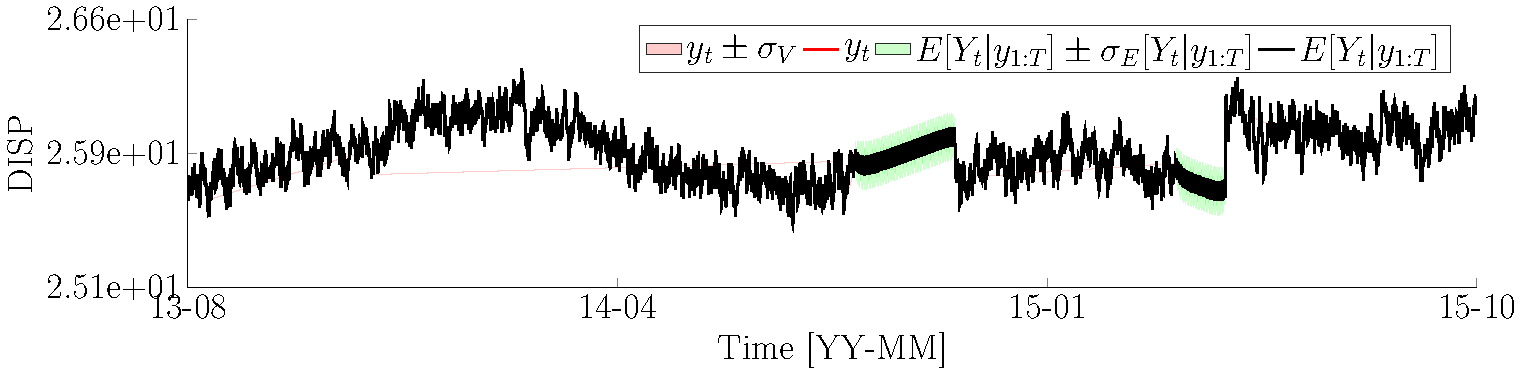
\includegraphics[width=0.9\linewidth]{./docfigs/Example_DISP_INTERVENTION/DISP_ObservedPredicted.pdf} 
\caption{Observed and estimated displacement data}
\end{subfigure}
\begin{subfigure}{\linewidth}
\centering
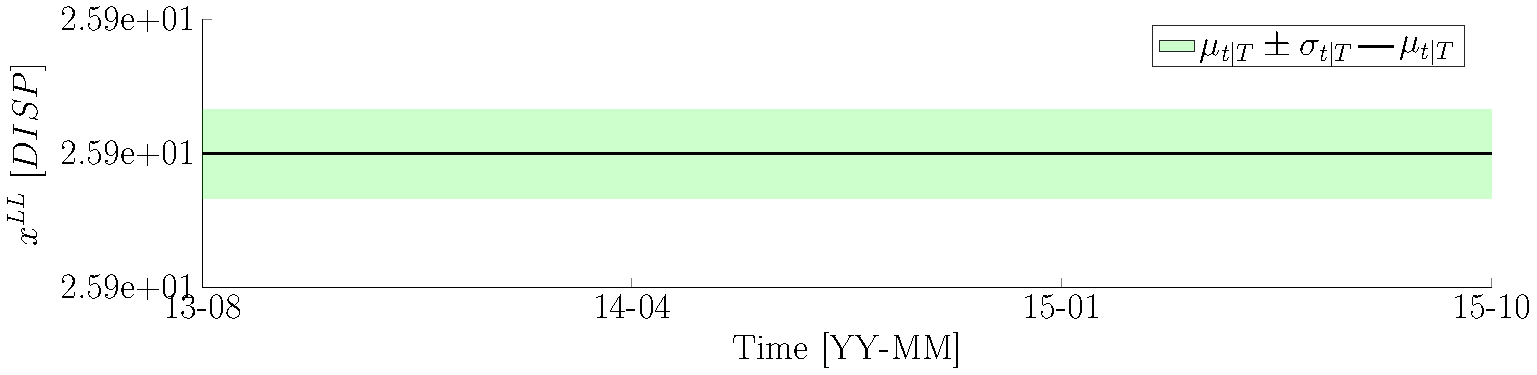
\includegraphics[width=0.9\linewidth]{./docfigs/Example_DISP_INTERVENTION/DISP_LL_1.pdf}
\caption{Estimated displacement local level component.}
\end{subfigure}
\begin{subfigure}{\linewidth}
\centering
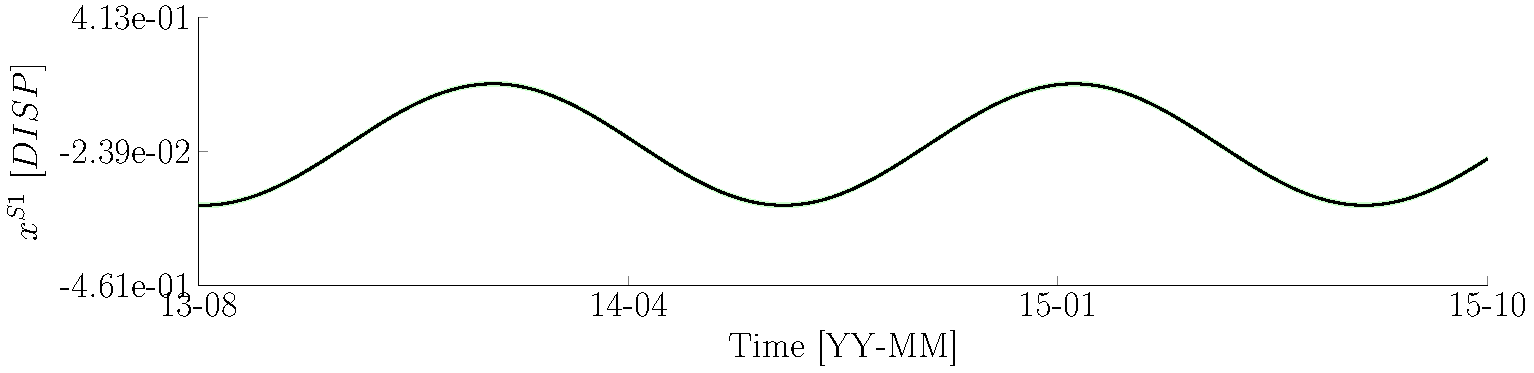
\includegraphics[width=0.9\linewidth]{./docfigs/Example_DISP_INTERVENTION/DISP_S1_2.pdf} 
\caption{Estimated displacement yearly periodic component (first hidden state)}
\end{subfigure}
\begin{subfigure}{\linewidth}
\centering
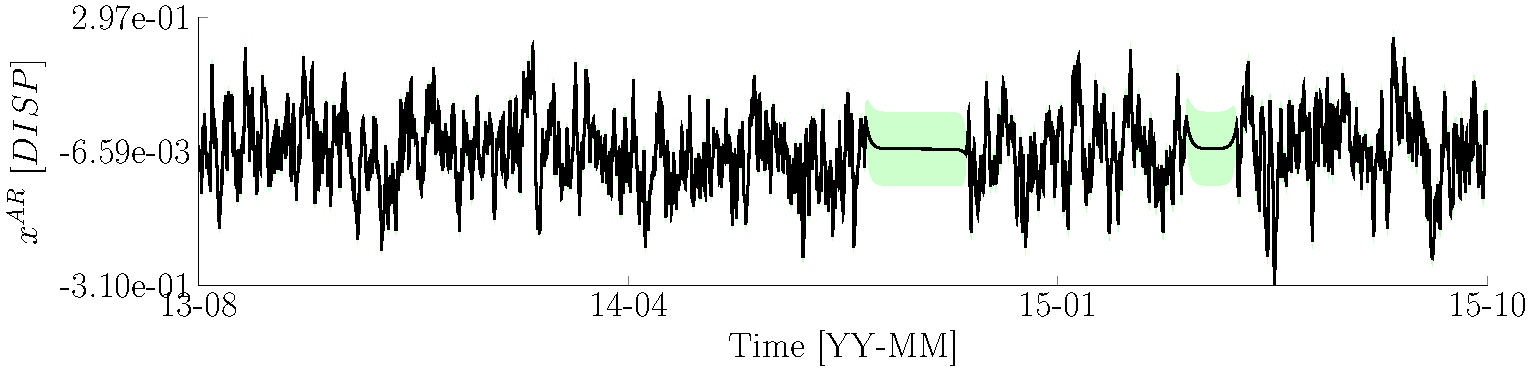
\includegraphics[width=0.9\linewidth]{./docfigs/Example_DISP_INTERVENTION/DISP_AR_6.pdf} 
\caption{Estimated displacement autoregressive component}
\end{subfigure}
\begin{subfigure}{\linewidth}
\centering
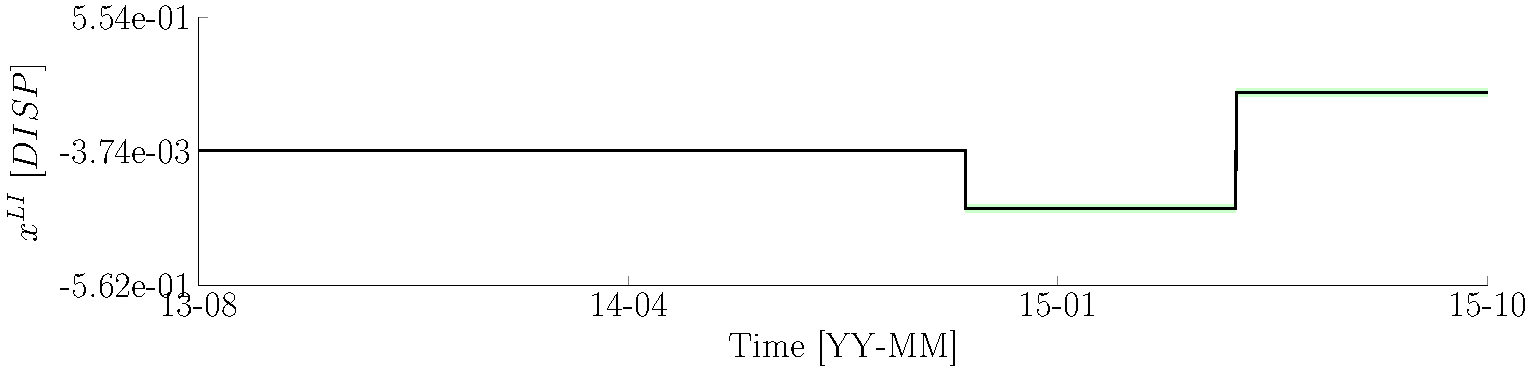
\includegraphics[width=0.9\linewidth]{./docfigs/Example_DISP_INTERVENTION/DISP_LI_7.pdf}
\caption{Estimated displacement daily periodic component (first hidden state)}
\end{subfigure}
\caption{Estimated results using OpenBDLM with the optimized model parameters and estimated initial hidden states. The hidden states are estimated from the data presented in Figure~\ref{fig:DataSummary1}a. The solid line and shaded area represent the mean and standard deviation of the estimated hidden states.}
\label{fig:Example_DISP_INTERVENTIONOptimizedOptimizedExample1}
\end{center}
\end{figure*}



